\chapter{Intégrales multiples}
\section{tribu produit}
\begin{mandatory}
\begin{defn}
Soient deux espaces mesurables $(E, \mathcal{T})$,$(F, \mathcal{F})$. La tribu
produit sur $E\times F$ est la plus petite tribu rendant les projections
canoniques $\pi_E,\pi_F$ mesurables. On la note $\mathcal{T}\otimes
\mathcal{F}$.
\end{defn}
\end{mandatory}
Il est possible de caractériser de façon simple cette tribu: pour que la
projection $\pi_E$ (resp. $\pi_F$) soit mesurable, il faut que pour tout $A \in
\mathcal{T}$ (resp. $B \in \mathcal{F}$) l'image réciproque $\pi^{-1}(A) = A
\times F$ (resp. $\pi_F^{-1}(B) = E \times B$) soit dans $\mathcal{T}\otimes \mathcal{F}$.
Par intersection entre ensembles de la forme précédente, on en déduit que tous
les produits cartésiens $A \times B$ avec $A \in
\mathcal{T}$, $B \in \mathcal{F}$ sont dans $\mathcal{T}\otimes \mathcal{F}$.
Cette tribu contient donc la tribu engendrée par ces produits cartésiens.
Réciproquement, la tribu engendrée par les produits cartésiens contient les
ensembles de la forme $A \times F$, $E \times B$, donc rend les projections
canoniques mesurables et contient ainsi $\mathcal{T}\otimes \mathcal{F}$: les
deux tribus sont donc égales.
\begin{defn}
Soient $E,F$ deux ensembles. Soit $A \subset E \times F$. Soit $x \in
E$ (resp $y \in F$) La section de $A$ selon $x$
(resp. $y$) est l'ensemble $A_x \subset F$ (resp $A^y \subset E$) defini par~:
\[
A_x = \{ v \in F | (x,v) \in A \}
\]
resp.
\[
A^y = \{ u \in E | (u,y) \in A \}
\]
\end{defn}
Pour une application $f$ définie sur $E \times F$, on construira de même
les sections~:
\[
f_x : v \in F  \to f(x,v) \, \quad f^y : u \in E \to f(u,y)
\]
\begin{prop}
Soit $(E, \mathcal{T}), (F, \mathcal{F})$ deux espaces mesurables avec
$\mu,\nu$ mesures $\sigma$-finies. 
\begin{itemize}
\item Si $A \subset E \times F$ appartient à la tribu produit
$\mathcal{T} \otimes \mathcal{F}$ alors les sections $A_x,A^y$ sont
respectivement $\mathcal{F}$ et $\mathcal{T}$ mesurables pour toute
valeur de $x$ et $y$.
\item Si $f$ est une application définie sur $E \times F$ et
mesurable, alors ses sections sont mesurables.
\end{itemize}
\end{prop}
\begin{proof}
La preuve utilise un classique argument de minimalité. Soit $x  \in E$
et soit $\mathcal{G} = \{ A \in \mathcal{T} \times \mathcal{F} | A_x
\in \mathcal{F} \}$. On a~:
\begin{itemize}
\item $\emptyset \in \mathcal{G}$.
\item $E \times F \in \mathcal {G}$.
\end{itemize}
de plus, $(A_x)^c = A^c_x$ d'où la stabilité de $\mathcal{G}$ par
passage au complémentaire. Enfin, pour toute famille dénombrable
$(A_n)$ d'éléments de $\mathcal{G}$, $(\cup_n A_n)_x = \cup_n
(A_n)_x$. L'ensemble $\mathcal{G}$ est donc une tribu. Elle contient
tous les rectangles $A \times B$ avec $A\in \mathcal{T}, B \in
\mathcal{F}$. Par minimalité de la tribu produit, elle contient donc
$\mathcal{T} \otimes \mathcal{F}$. 
La proposition relative aux sections d'applications en découle immédiatement.
\end{proof}
\section{Théorème de Fubini}

\begin{prop}
Soient $(E, \mathcal{T}, \mu), (F, \mathcal{F}, \nu)$ deux espaces
mesurés avec $\mu,\nu$ mesures $\sigma$-finies. 
Si $A \in \mathcal{T} \times \mathcal{F}$, l'application $x
\to \nu(A_x)$ (resp. $y \to \mu(A^y)$) est mesurable.
\end{prop}
\begin{proof}
Supposons tout d'abord que la mesure $\nu$ soit finie. Soit
$\mathcal{G} = \{ A \in \mathcal{T} \times \mathcal{F} | x \to
\nu(A_x) \mbox { mesurable } \}$. Tous les rectangles de la forme  $A
\times B$ avec $A\in \mathcal{T}, B \in \mathcal{F}$ sont dans
$\mathcal{G}$ car $\nu((A \times B)_x) = \nu(B) 1_A(x)$. Soient $A,B
\in \mathcal{G}$ avec $A \subset B$. On a $\nu((B-A)_x) = \nu(B_x) -
\nu(A_x)$ donc $A - B \in \mathcal{G}$. Si $(A_n)$ est une famille
dénombrable croissante d'éléments de $\mathcal{G}$, comme~:
\[
\nu((\cup_n(A_n))_x) = \nu(\cup_n (A_n)_x) = \lim_n \nu((A_n)_x)
\]
on a $\cup_n A_n \in \mathcal{G}$. L'ensemble $\mathcal{G}$ est une
classe monotone. On vérifie qu'elle est stable par intersections
finies, ce qui montre qu'elle est égale à la tribu $\mathcal{T} \times
\mathcal{G}$ d'où la proposition. 
Si la mesure est $\sigma$-finie, on étend le résultat obtenu en
prenant un recouvrement dénombrable par des ensembles de $\nu$-mesure finie.
\end{proof}
\begin{mandatory}
\begin{theorem}
Sous les hypothèses de la proposition précédente, il existe une unique
mesure sur $\mathcal{T} \otimes \mathcal{F}$, notée $\mu \otimes \nu$,
telle que $\mu\otimes \nu (A \times B) = \mu(A) \nu(B)$ pour $A \in
\mathcal{T}, B \in \mathcal{F}$. De plus, on a~:
\[
\forall A \in \mathcal{T} \otimes \mathcal{F} \, , \mu \otimes \nu (A) = \int_E
\nu(A_x) d \mu = \int_F \mu(A^y) d \nu
\]
\end{theorem}
\end{mandatory}
\begin{proof}
La démonstration est élémentaire dès lors que la proposition
précédente est prouvée et est laissée à titre d'exercice.
\end{proof}
Dans le cas où $\mu$ et $\nu$ sont égales à la mesure de Lebesgue sur
$\mathbb{R}$, la mesure produit est la mesure de Lebesgue sur $\mathbb{R}^2$ qui
à un produit cartésien d'intervalles associe sa surface. On peut étendre sans
difficulté ce résultat à $\mathbb{R}^n$.
\begin{mandatory}
\begin{theorem}(Tonnelli)
Soient $(E, \mathcal{T}, \mu), (F, \mathcal{F}, \nu)$ deux espaces
mesurés avec $\mu, \nu$ mesures $\sigma$-finies et soit $f : E \times F \to \mathbb{R}^+$ une application
mesurable. 
\begin{itemize}
\item L'application $x \to  \int_F f_x d \nu $ (resp. $y \to
\int_E f^y d \mu$) est mesurable.
\item On a:
 \begin{align*}
\int_{E \times F} f d( \mu \otimes \nu) & = \int_E \left (
\int_F f_x d \nu \right ) d \mu \\
& = \int_F \left (
\int_E f^y d \mu \right ) d \nu
\end{align*}
\end{itemize}
\end{theorem}
\end{mandatory}
\begin{proof}
Le théorème est immédiat si $f = 1_A$ avec $A \in \mathcal{T} \times
\mathcal{F}$. Par linéarité de l'intégrale, il reste vrai sur les
applications étagées positives, puis, par convergence monotone sur
toutes les applications mesurables positives.
\end{proof}
Comme dans pratiquement tous les cas en théorie de Lebesgue, il faut traiter
séparément le cas des applications de signe quelconque, en adjoignant
l'hypothèse de sommabilité. Le théorème suivant est souvent appliqué en ayant au
préalable utilisé le théorème de Tonnelli sur la valeur absolue de l'application
à intégrer.
\begin{mandatory}
\begin{theorem}(Fubini)
Soient $(E, \mathcal{T}, \mu), (F, \mathcal{F}, \nu)$ deux espaces
mesurés et avec $\mu,\nu$ mesures $\sigma$-finies. Soit $f : E \times F \to
\mathbb{R}$ une application sommable par rapport à $\mu \otimes \nu$.
\begin{itemize}
\item Pour $\mu$-presque tout $x\in E $ (resp. $\nu$-presque tout $y
\in  F$), l'application $f_x$ (resp. $f^y$) est sommable.
\item En posant~:
\[
I : x \to \left \{
\begin{array}{cc}
\int_F f_x d \nu & \mbox { si } f_x \mbox { sommable } \\
0 & \mbox{ sinon }
\end{array}
\right .
\]
\[
J : y \to \left \{
\begin{array}{cc}
\int_E f^y d \mu & \mbox { si } f^y \mbox { sommable } \\
0 & \mbox{ sinon }
\end{array}
\right .
\]
on a~:
\[
\int_{E \times F} f d (\mu \otimes \nu) = \int_E I(x) d \mu(x) = \int_F J(y)
d \nu(y)
\]
\end{itemize}
\end{theorem}
\end{mandatory}
\begin{proof}
Soit $f^+$ (resp. $f^-$) la partie positive (resp. négative) de
$f$. Les sections $f^+_x$ et $f^-_x$ sont mesurables et par le
théorème de Tonnelli les applications~:
\[
x \to \int_F f^+_x d \nu \, , x \to  \int_F f^-_x d \nu
\]
sont sommables. On en déduit qu'elles sont finies $\mu$-presque partout
et donc que $I$ est $\mu$-sommable. 
Le théorème est obtenu en écrivant~:
\begin{align*}
\int_{E \times F} f d (\mu \otimes \nu) & = \int_{E \times F} f^+ d( \mu
\otimes \nu) - \int_{E \times F} f^- d (\mu \otimes \nu) \\
& = \int_E \left ( \int_F F^+_x d\nu \right ) d \mu -  \int_E \left (
\int_F F^-_x d\nu \right ) d \mu \\
& = \int_E I d \mu 
\end{align*}
\end{proof}
\begin{rem}
L'hypothèse de $\mu \otimes \nu$ sommabilité est fondamentale dans le
théorème de Fubini. Comme mentionné plus haut, on applique le plus souvent le
théorème de Tonnelli à $|f|$ pour pouvoir la montrer.
\end{rem}
Il est d'usage courant de simplifier l'écriture $d(\mu \otimes \nu)$ par $d\mu
d\nu$ en précisant éventuellement les variables d'intégration en argument de
$d\mu$ et $d\nu$. Il ne faut pas oublier néanmoins qu'il s'agit bien de la mesure produit.
\begin{exercice}
Soit la partie $D=[-1,+1]^2$ de $\mathbb{R}^2$. Calculer les intégrales~:
\[
\int_{D} (x^2 +y^2) d \lambda d\lambda \quad, \quad  \int_{D} y e^{xy} d
\lambda d \lambda
\]
\end{exercice}
\begin{exercice}
On dit qu'une application $f : \mathbb{R} \to \mathbb{R}$ est
localement intégrable si elle est sommable sur tout compact de
$\mathbb{R}$. Soient $f,g$ localement intégrables. On pose~:
\[
F : x \to \int_0^x f(t) d \lambda(t) , \quad G : x \to \int_0^x g(t) d
\lambda(t)
\]
\begin{itemize}
\item Montrer, en utilisant l'application~:
\[
h : (x,y) \to 1_{x \leq y} g(x) f(y)
\]
que pour tout intervalle borné $[a,b]$~:
\[
\int_{[a,b]} f(t)(G(t) - G(a)) d\lambda(t) =
\int_{[a,b]}g(t)(F(b)-F(t)) d\lambda(t)
\]
\item En déduire la formule d'intégration par parties~:
\[
\int_{[a,b]} F(t) g(t) d \lambda(t) = F(b)G(b)-F(a)G(a) - \int_{[a,b]}
f(t) G(t) d \lambda(t)
\]
\end{itemize}
\end{exercice}

Attention à l'hypothèse de sommabilité dans Fubini, m\^eme si tout semble
marcher:
\begin{exercice}
On se place sur le même domaine $D$ qu'à l'exercice 12. Soit~:
\[
f : (x,y) \to \frac{xy}{(x^2+y^2)^2}
\]
\begin{itemize}
\item Calculer~:
\[
\int_{[-1,+1]} \left ( \int_{[-1,+1]} f(x,y) d \lambda(x) \right )
d \lambda(y)
\]
et
\[
\int_{[-1,+1]} \left ( \int_{[-1,+1]} f(x,y) d \lambda(y) \right )
d \lambda(x)
\]
\item Peut-on en déduire, par le théorème de Fubini, la valeur de~:
\[
\int_D f(x,y) d \lambda d \lambda
\]
\end{itemize}
\end{exercice}

\section{Changement de variable}

La formule du changement de variable par les $C^1$-difféomorphismes 
dans $\mathbb{R}^n$ est d'une grande importance tant pratique que
théorique. 
Elle est essentiellement basée sur un calcul de
changement de volume pour des cubes élémentaires, puis l'utilisation
du théorème des classes monotones pour passer à des boréliens
quelconques.
Dans la suite on supposera toujours que l'on travaille dans
$\mathbb{R}^n$ muni de sa topologie usuelle.
La première proposition qui va être montrée maintenant est essentiellement une
traduction en terme de mesure image de la propriété géométrique bien connue
selon laquelle le volume d'un parallélépipède de $\mathbb{R}^n$ qui s'appuie sur
les $n$ vecteurs $v_1,\dots v_n$ est donné par $|\det(v_1,\dots,v_n)|$.
\begin{mandatory}
\begin{prop}
Soit $f \colon \mathbb{R}^n \to \mathbb{R}^n$ une application linéaire
inversible de matrice représentative $M$. Pour tout borélien $B$, on
a~:
\[ 
\lambda(f(B)) = |\det(M)| \lambda(B)
\]
\end{prop}
\end{mandatory}
On remarquera que l'application $B \to \lambda(f(B))$ est la mesure
image de $\lambda$ par $f^{-1}$.
\begin{proof}
Soit $B$ un borélien. Pour tout $x \in \mathbb{R}^n$, on a~:
\[
\lambda(f(B + x)) = \lambda(f(B) + f(x)) = \lambda(f(x))
\]
On en déduit que la mesure image de $\lambda$ par $f^{-1}$ est
invariante par translation, donc égale, à une constante multiplicative
près, à la mesure de Lebesgue~:
\[
\exists C >0 \, | \, \forall B \in \mathcal{B}(\mathbb{R}^n), \, \lambda(f(B)) =
C \lambda(B)
\]
Supposons dans un premier temps $M$ orthogonale. La boule unité est
laissée invariante par $f$, d'où $C = 1 = |\det(M)|$ dans ce cas. Supposons
maintenant que $M$ est diagonale, à coefficients diagonaux $\sigma_i,
i=1\dots n$ positifs. L'image de $[0,1]^n$ est $\prod_{i=1\dots n}
[0, \sigma_i]$, d'où l'on déduit $C = \prod_{i=1\dots n} \sigma_i =
|\det(M)|$. Dans le cas général, on applique les deux résultats
précédents à la décomposition en valeurs singulières $M = U \Sigma
V^t$ de $M$, où les deux matrices $U,V$ sont orthogonales et la matrice $\Sigma$
est diagonale.
\end{proof}
\begin{defn}
Une application inversible $f : \mathbb{R}^n \to \mathbb{R}^n$ est
appelée $C^k$-difféomorphisme si elle est de classe $C^k$ ainsi que
son inverse.
\end{defn}
\begin{term}
Soit $f$ une application différentiable . L'application
jacobienne (ou Jacobien) est l'application $J_f : x \to det(f^\prime(x))$. 
\end{term}
Lorsque une application est de classe $C^1$, elle est bien approchée par son
application dérivée au voisinage d'un point quelconque: on peut donc espérer
que la mesure image associée à $f$ ne soit pas très différente de celle
correspondant à l'approximation linéaire de $f$ en chaque point. Cette
situation est résumée en figure \ref{ch3:2}.  
\begin{figure}[h]
 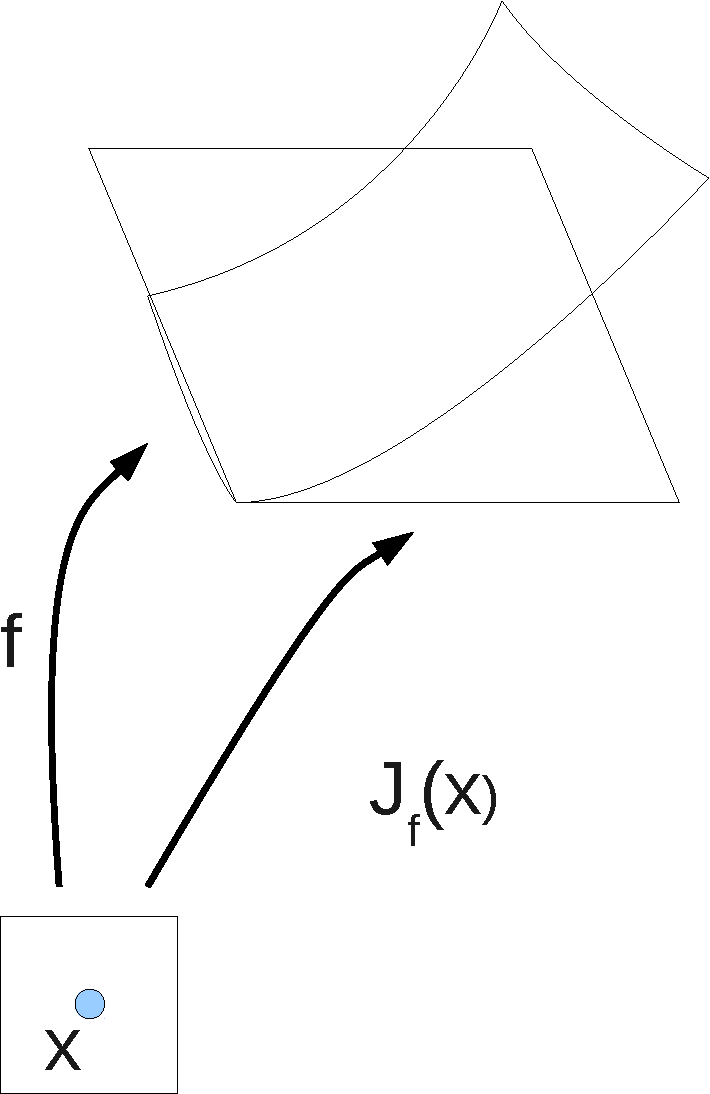
\includegraphics[scale=0.3]{images/jacobien.pdf}
\caption{Volume image et volume image approché}\label{ch3:2}
\end{figure}
La proposition suivante va prouver
que dans le cas simple des cubes, la différence entre les deux peut être bornée, 
et rendue aussi petite que l'on souhaite en restreignant
la taille des cubes considérés. 
\begin{prop}
Soit $U,V$ deux ouverts de $\mathbb{R}^n$ et $K$ un compact de $U$. Soit $f : U \to V$ un
$C^1$-difféomorphisme. Pour tout $\epsilon > 0$, il existe $\delta >
0$ tel que pour tout cube $C$ de centre $x_0 \in K$ dont la longueur du
côté est inférieure à $\delta$~:
\[
(1-\epsilon)^n |J_f(x_0)| \lambda(C) \leq \lambda(f(C)) \leq (1+\epsilon)^n
|J_f(x_0)| \lambda(C)
\]
\end{prop}
\begin{proof}
Par hypothèse, $f^\prime$ est continue, il existe donc $\delta > 0$
tel que~:
\[
\| x - x_0 \| < \delta \rightarrow \| f^\prime(x) - f^\prime(x_0) \| < \epsilon
\]
On peut choisir $\delta$ suffisamment petit pour que  $C \subset K$
et que la propriété ci-dessus soit vraie. 
Pour tout $x \in C$, il existe $c \in C$ tel que $f(x) - f(x_0) =
f^\prime(c) (x-x_0)$. En combinant ce résultat avec le précédent, on
en déduit~:
\[
\| f(x) - f(x_0) - f^\prime(x_0)(x-x_0)\| \leq \epsilon \|x-x_0\|
\]
Soit l'application affine~:
\[
T : x \to f(x_0)+f^\prime(x_0)(x-x_0)
\]
On peut écrire, pour $x \in C$~:
\[
f(x) = T(x + T^{-1}g(x,x_0))
\]
avec $\| g(x,x_0) \| \leq \epsilon \|x -x_0\|$.
En posant~:
\[
\eta = \sup \{ \| f^{\prime}(x)^{-1} \|, x \in K \}
\]
il vient~:
\[
\|  T^{-1}g(x,x_0) \| \leq \eta \epsilon \| x - x_0 \|
\]
et donc~:
\[
\lambda(f(C)) \leq \lambda(T((1+\eta \epsilon )C)) =
(1+\eta\epsilon)^n |J_f(x_0)| \lambda(C)
\]
On montrerait de même la minoration.
\end{proof}
\begin{defn}
Un cube élémentaire d'ordre $k \geq 1$ est un cube de la forme~:
\[
C = \prod_{i=1}^n [ x_i 2^{-k}, (x_i + 1)2^{-k} ]
\]
où les $x_i, i=1\dots n$ sont des entiers.
\end{defn}
En recouvrant un cube élémentaire $C$ d'ordre $k$ quelconque par des
cubes vérifiant les hypothèses de la proposition précédente pour
$\epsilon > 0$ donné, on obtient (exercice)~:
\[
(1-\epsilon)^2 \int_{C} |J_f(x)|d \lambda(x) \leq \lambda(f(C)) \leq
(1+\epsilon)^2 \int_{C} |J_f(x)| d \lambda(x)
\]
puis l'égalité par passage à la limite. 
\begin{mandatory}
\begin{prop}
Soient $U,V$ ouverts de $\mathbb{R}^n$. Soit $f : U \to V$ un
$C^1$-difféomorphisme. On a, pour tout borélien $B$~:
\[
\lambda(f(B)) = \int_B |J_f(x) |d \lambda(x)
\]
\end{prop}
\end{mandatory}
\begin{proof}
Les cubes élémentaires d'adhérence incluse dans $U$ forment une
classe monotone $\mathcal{C}$. La mesure  $\lambda(f(C))$ d'un cube
$C$ de cette classe est égale à $ \int_C |J_f(x) |d \lambda(x)$. Le
résultat se déduit du théorème des classes monotones en remarquant que
$\mathcal{C}$ est stable par intersections finies et engendre la tribu
de Borel.
\end{proof}
\begin{rem}
 L'extension de la proposition au cas des $C^1$-difféo\-morphismes par
morceaux se fait immédiatement en l'appliquant sur une partition de
$U$.
\end{rem}
\begin{mandatory}
\begin{prop}{(Changement de variable)}
Sous les hypothèses précédentes, on a, pour toute application $g : V
\to \mathbb{R}$~:
\[
\int_V g(x) d \lambda(x) = \int_U g(f(x)) |J_f(x)| d \lambda(x)
\]
\end{prop}
\end{mandatory}
\begin{rem}
La proposition est une conséquence immédiate du résultat sur la mesure
image. Pour une application $g$ de signe quelconque, on utilisera souvent
la formule ci-dessus sur $|g|$ pour montrer la sommabilité, puis à
nouveau sur $g$ pour calculer l'intégrale (en toute rigueur pour
$g^+,g^-$, mais un calcul élémentaire montre que cela revient au même).
\end{rem}
La technique du changement de variable est à connaître absolument: c'est une
des méthodes de base pour calculer une valeur d'intégrale.
\begin{exercice}
Soit l'application $f : \mathbb{R}^{+2} \to \mathbb{R}^+$ définie par~:
\[
f : (x,y) \to e^{-x^2 -y^2}
\]
\begin{itemize}
\item A l'aide du changement de variable~:
\[
\begin{array}{c}
x = \rho \cos \theta \\
y = \rho \sin \theta 
\end{array}
\]
où $\rho \in \mathbb{R}^+, \, \theta \in [0, \frac{\pi}{2}]$, calculer~:
\[
\int_{\mathbb{R}^{+2}} f(x,y) d \lambda(x) \times d \lambda(y)
\]
\item En déduire la valeur de~:
\[
\int_{\mathbb{R}} e^{-x^2} d \lambda (x)
\]
\end{itemize}
\end{exercice}
L'utilisation conjointe des théorèmes de Fubini-Tonnelli et du changement de
variable est fréquente. Dans l'exercice suivant, on établit une relation entre
des fonctions appelées fonctions eulériennes gamma et béta, qui sont d'un usage
assez courant.
\begin{exercice}
Soit $a>0, b>0$ deux réels strictement positifs. 
\begin{itemize}
  \item Montrer que les deux intégrales
suivantes sont bien définies:
\[
\Gamma(a) = \int_{\mathbb{R}^+} e^{-x}x^{a-1} d\lambda(x) \, , \, B(a,b) =
\int_{[0,1]} x^{a-1}(1-x)^{b-1} d \lambda(x)
\]
\item Montrer que:
\[
\Gamma(a) = 2 \int_{\mathbb{R}^+} e^{-x^2} x^{2a-1} d \lambda(x)
\]
\item Justifier avec précision que:
\[
\Gamma(a)\Gamma(b) = 4 \int_{\mathbb{R}^{+2}}
e^{-(x^2+y^2)}x^{2a-1}y^{2a-1}d\lambda(x) d\lambda(y)
\]
\item En utilisant le changement de variable de l'exercice précédent, en
déduire:
\[
\Gamma(a)\Gamma(b)=B(a,b)\Gamma(a+b)
\]
\end{itemize}

\end{exercice}
